\begin{center}
  \Large
  \textbf{BIOGRAFI PENULIS}
\end{center}

\addcontentsline{toc}{chapter}{BIOGRAFI PENULIS}

\vspace{2ex}

\begin{wrapfigure}{L}{0.3\textwidth}
  \centering
  \vspace{-3ex}
  % Ubah file gambar berikut dengan file foto dari mahasiswa
  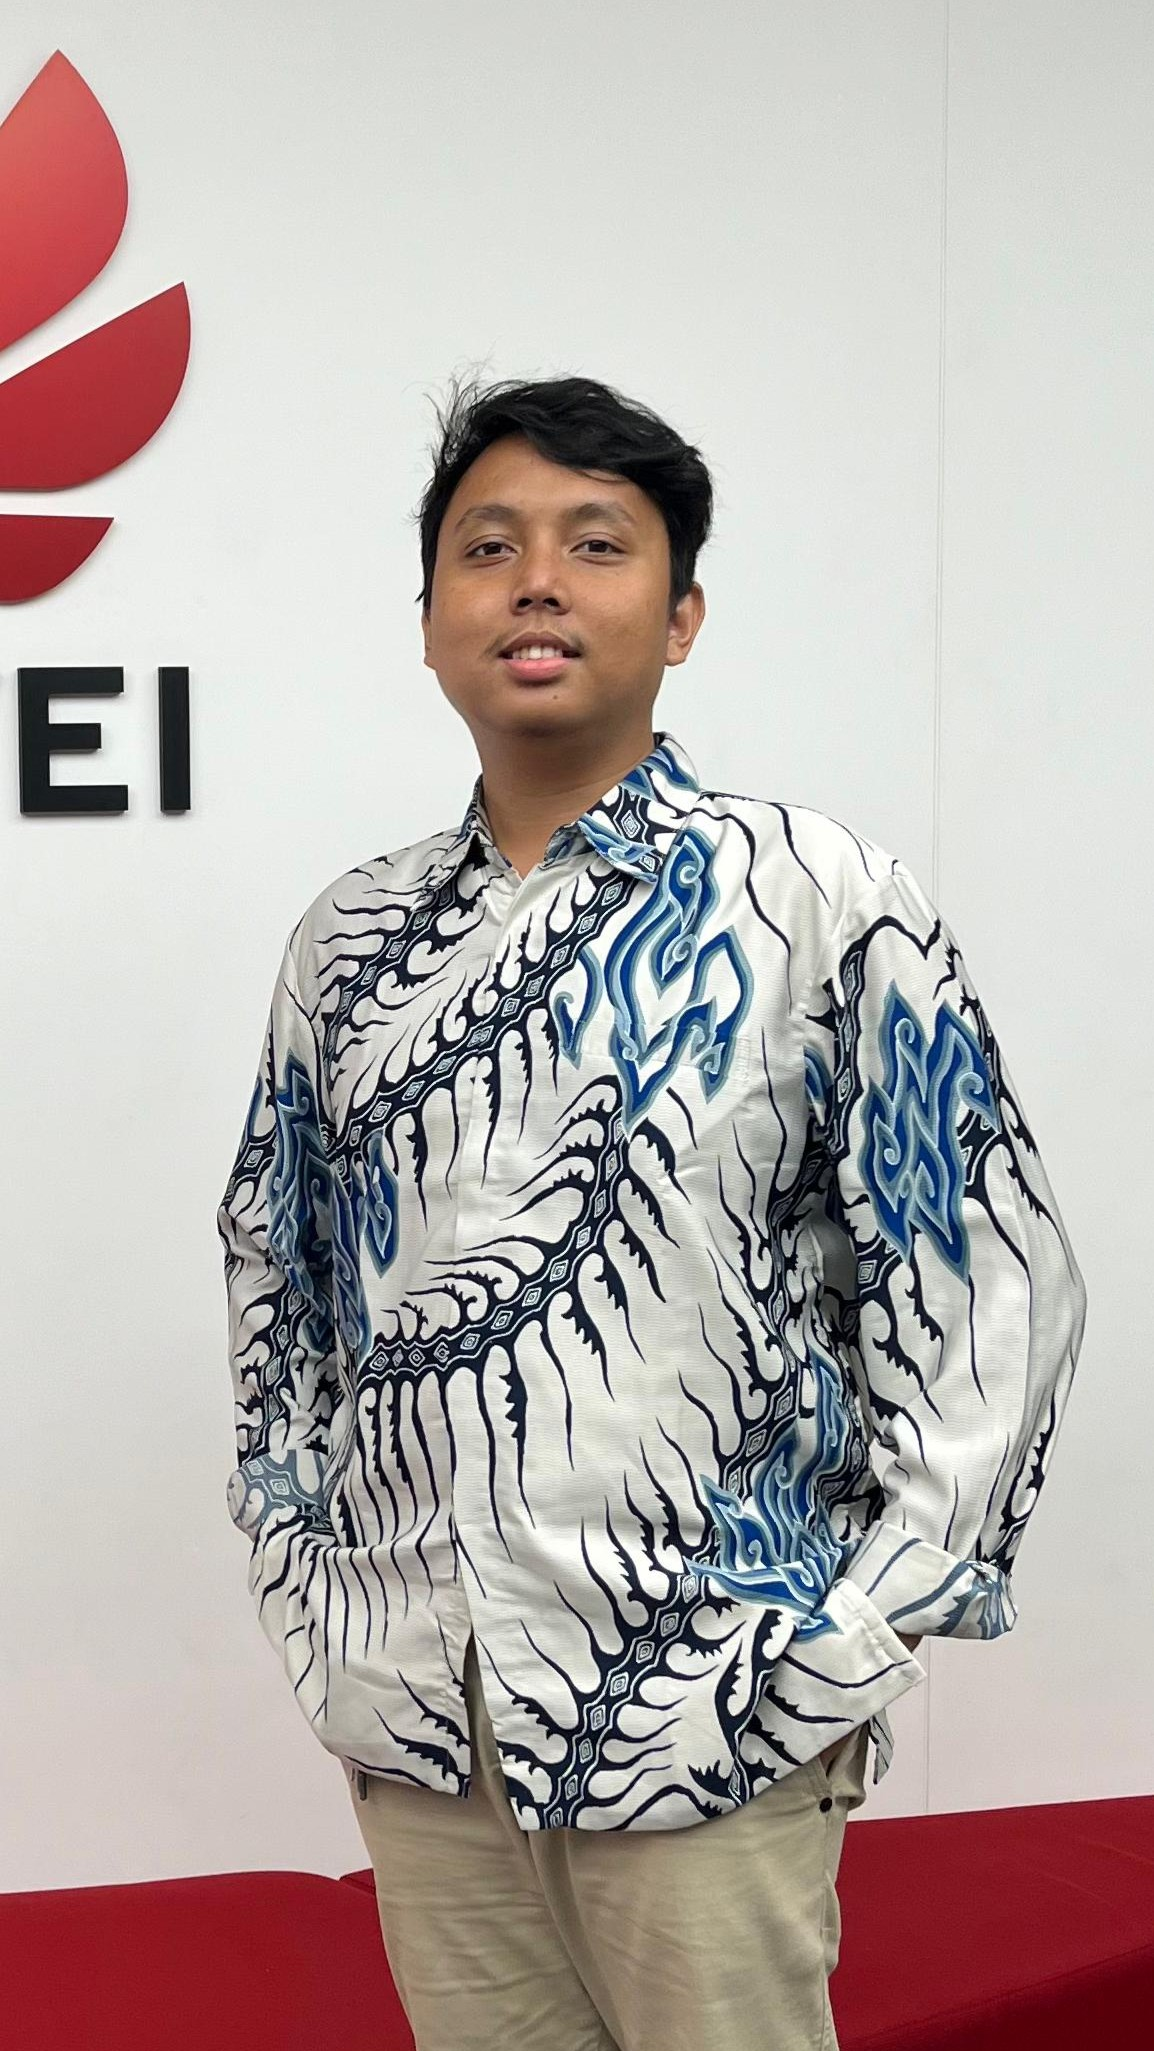
\includegraphics[width=0.3\textwidth]{gambar/Dzakirozaan Uzlahwasata.jpg}
  \vspace{-4ex}
\end{wrapfigure}

% Ubah kalimat berikut dengan biografi dari mahasiswa
\name{}, lahir di Yogyakarta pada tanggal 16 Februari 2003. Penulis menempuh pendidikan dasar di SD Muhammadiyah Sleman, melanjutkan pendidikan menengah pertama di SMPN 4 Pakem, dan menamatkan pendidikan menengah atas di SMAN 1 Teladan Yogyakarta. Pada tahun 2021, penulis secara resmi terdaftar sebagai mahasiswa Program Studi Teknologi Informasi di Institut Teknologi Sepuluh Nopember.

Selama masa perkuliahan, penulis aktif berkontribusi dalam berbagai kegiatan organisasi, kepanitiaan, dan pengembangan diri. Penulis mengawali keterlibatannya dengan menjadi Wakil Ketua di Ini Lho ITS! Region Yogyakarta pada tahun 2021. Selanjutnya, penulis aktif di BEM FTEIC ITS, sebagai \textit{Staff Internal Affairs} pada periode 2023-2024. Penulis juga dipercaya memegang peran dalam berbagai kepanitiaan kampus, seperti Wakil Ketua Region di GERIGI ITS 2023 dan Ketua Divisi Acara di ARA 5.0. Di samping itu, penulis juga mendapatkan amanah sebagai Kepala Divisi pada Riset dan Teknologi BEM FTEIC ITS periode 2024-2025.

Untuk mendalami minat dan keahlian di bidang \textit{Cloud Computing} dan \textit{Software}, penulis berpartisipasi dalam program Studi Independen Bersertifikat Kampus Merdeka di Bangkit Academy by Google, GoTo, Traveloka pada jalur pembelajaran \textit{Cloud Computing Path}. Pengalaman ini diperkuat dengan pengalaman kerja profesional melalui program magang sebagai \textit{Software Engineer} di PLN Nusantara Power Services dan sebagai \textit{Assistant Project Controller} di Huawei.

Di luar kegiatan organisasi dan profesional, penulis juga aktif sebagai bentuk kontribusi di lingkungan akademik, penulis dipercaya menjadi asisten dosen untuk mata kuliah Sistem Operasi dan Arsitektur \textit{Enterprise}.